\documentclass[12pt]{article}
\usepackage{subfiles}
\usepackage{graphicx}
\usepackage[
        pdfencoding=auto,%
        pdfauthor={Scott Pratt},%
        pdfstartview=FitV,%
        colorlinks=true,%
        linkcolor=blue,%
        citecolor=blue, %
        urlcolor=blue,
        breaklinks=true]{hyperref}
%\usepackage[anythingbreaks,hyphenbreaks]{breakurl}
\usepackage[anythingbreaks,hyphenbreaks]{xurl}
%\usepackage{pdfsync}
\usepackage{amssymb}
\usepackage{amsmath}
\usepackage{bm}
\numberwithin{equation}{section} 
\numberwithin{figure}{section} 
\usepackage[small,bf]{caption}
%\usepackage{fontspec}
%\usepackage{textcomp}
%\usepackage{color}
\usepackage{fancyhdr}
\setlength{\headheight}{16pt}
%\usepackage[headheight=110pt]{geometry}
\usepackage{bm}

\usepackage[most]{tcolorbox}
\tcbset{
frame code={}
center title,
left=0pt,
right=0pt,
top=0pt,
bottom=0pt,
colback=gray!25,
colframe=white,
width=\dimexpr\textwidth\relax,
enlarge left by=0mm,
boxsep=5pt,
arc=0pt,outer arc=0pt,
}
\newcounter{examplecounter}
\counterwithin{examplecounter}{section}
\setcounter{examplecounter}{0}
\newcommand{\example}[2]{\begin{tcolorbox}[breakable,enhanced]
\refstepcounter{examplecounter}{
\bf Example \arabic{section}.\arabic{examplecounter}:}~~{\bf #1}\\
{#2}
\end{tcolorbox}
}
%\newcommand{\exampleend}{
%\begin{samepage}
%\nopagebreak\noindent\rule{\textwidth}{1pt}
%\end{samepage}
%}


%\usepackage{silence}
%\WarningFilter{hyperref}{Token not allowed in a PDF String}

\newcommand\eqnumber{\addtocounter{equation}{1}\tag{\theequation}}

\newcommand{\solution}[1]{ }



\usepackage{comment}
\parskip 4pt
\parindent 0pt

%\newcommand{\bm}{\boldmath}
\boldmath

%

\begin{document}

\today\\

\centerline{\bf\Large Proton-Deuteron Correlations}
\centerline{Scott Pratt, prattsc@msu.edu}

Correlations are calculated by convoluting wave functions with source functions, $S(\vec{V},\vec{r})$, with the relative wave function, $\phi_{\vec{q}}(\vec{r})$, through the Koonin formula:
\begin{eqnarray}
C(\vec{V},\vec{q})&=&\int d^3r |\phi_{\vec{q}}(\vec{r})|^2 S(\vec{V},\vec{r}),\\
\nonumber
S(\vec{V},\vec{r})&=&\left.\frac{\int d^3r_ad^3r_b~f_a(\vec{V},\vec{r}_a,t)f_b(\vec{V},\vec{r}_b,t)\delta(\vec{r}_a-\vec{r}_b)}
{\int d^3r_ad^3r_b~f_a(\vec{V},\vec{r}_a,t)f_b(\vec{V},\vec{r}_b,t)}\right|_{t\rightarrow\infty},\\
\nonumber
\vec{V}&\equiv&\frac{\vec{p}_i}{E_i}
\end{eqnarray}
Here, $f_i(\vec{V},\vec{r},t)$ is the phase space density at asymptotic times for a particle of velocity $\vec{V}$ at position $\vec{r}$ and at time $t$. Evaluations of the phase-space density are performed in the center-of-mass frame. 

For the calculations performed here, $S(\vec{V},r)$ is simply assumed to have a Gaussian form, 
\begin{eqnarray}
S(\vec{V},\vec{r})&=&\frac{1}{(4\pi R^2)^{3/2}}e^{-r^2/4R^2}.
\end{eqnarray}
The relative momentum is the invariant relative momentum, i.e. in the center of mass frame, $\vec{q}_{\rm inv}=\vec{p}_a=-\vec{p}_b$. In this frame $q_{\rm inv}=\frac{1}{2}|(\vec{p}_a-\vec{p}_b|$. For such Gaussian fits the velocity $\vec{V}$ is irrelevant. 

The difficulty in pursuing these calculations derives from finding the wave function. For this case wave functions were found by solving the Schr\"odinger equation for the two particles under the influence of their Coulomb repulsion, plus their strong interaction. The form for the strong interaction was that of a sequence of square wells. Only the two $s-$wave channels were considered, $J=1/2$ and $J=3/2$. For $J=1/2$ three steps were used for the potential,\\
\begin{tabular}{|c|c|}
\hline
position (fm) & potential height (MeV)\\
\hline
$r<3.23445$ & -28.002\\
$3.23445<r<5.57680$ & 37.283\\
$5.57680<r<7.71351$ & -5.829\\
$r>7.71351$ & 0.0\\
\hline
\end{tabular}\\

For $J=3/2$ only one step was used,\\
\begin{tabular}{|c|c|}
\hline
position (fm) & potential height (MeV)\\
\hline
$r<4.99965$ & 108.203\\
$r>4.99965$ & 0.0\\
\hline
\end{tabular}

The potential parameters above were adjusted to fit phases shifts measured in \cite{Black:1999duc}. A plot of the phase shifts is given Fig. \ref{pdfitfig}. The phaseshift fitting only extended to relative momenta of 80 MeV/$c$, so any structure beyond that relative momenta was not incorporated into the analysis. The resulting correlations functions for several Gaussian sources are also shown in Fig. \ref{pdfitfig}.\\
\begin{figure}
\centerline{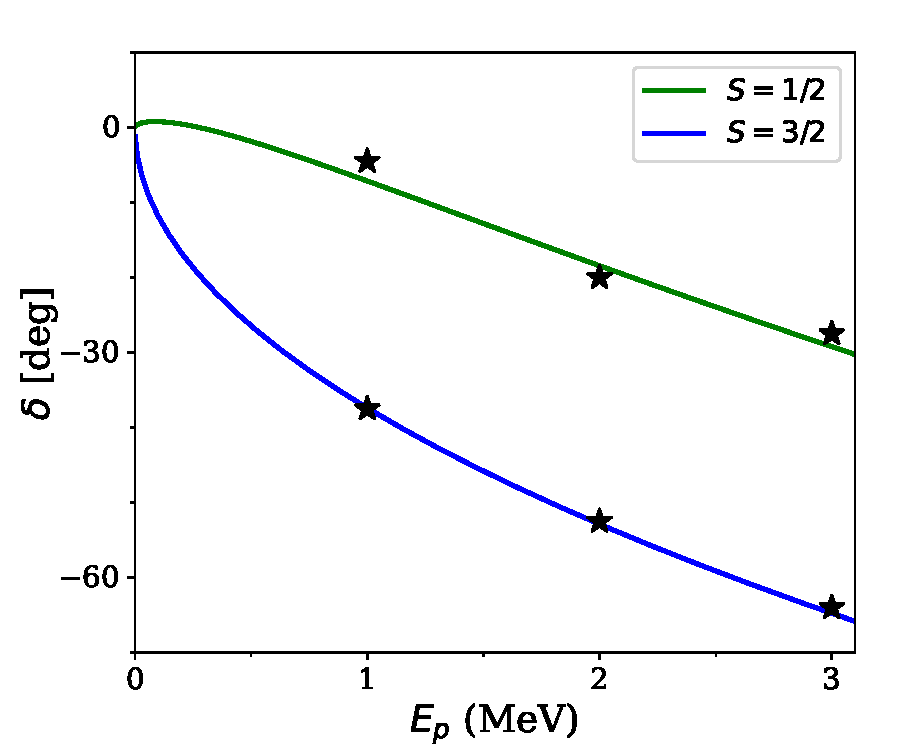
\includegraphics[width=3.0in]{phaseshifts_pd}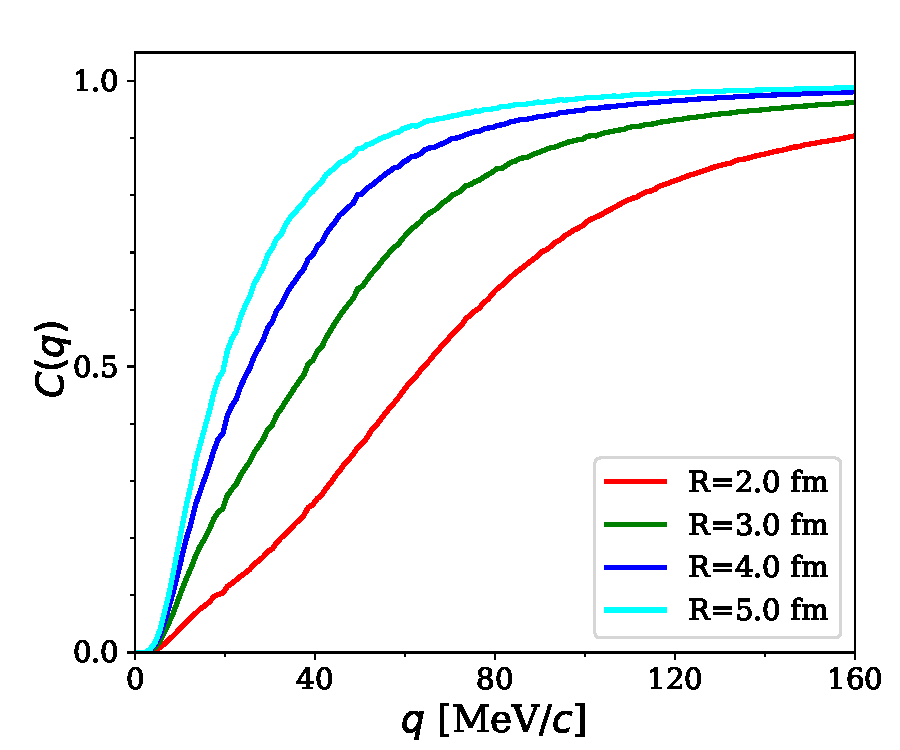
\includegraphics[width=3.0in]{cf_pd}}
\caption{\label{pdfitfig}
Left panel: Phase shifts for $pd$ as a function of the laboratory kinetic energy. The lines come from solving the Schr\"odinger equation for the two $s-$waves using the Coulomb interaction plus a multi-step step function form described above. The stars show experimental points taken from \cite{Black:1999duc}. The right-hand panel shows the resulting correlation functions for Gaussian sources of various sizes.}
\end{figure}

\begin{thebibliography}{99}
%\cite{Black:1999duc}
\bibitem{Black:1999duc}
T.~C.~Black, H.~J.~Karwowski, E.~J.~Ludwig, A.~Kievsky, S.~Rosati and M.~Viviani,
%``Determination of proton-deuteron scattering lengths,''
Phys. Lett. B \textbf{471}, 103-107 (1999).
%doi:10.1016/S0370-2693(99)01366-0
%16 citations counted in INSPIRE as of 24 Feb 2023
\end{thebibliography}








\end{document}
